\documentclass[xetex]{beamer}
\usepackage{fontspec}
\usepackage{xltxtra}
\usepackage{xunicode}
\usepackage{polyglossia}
%\usepackage[english]{babel}
\usepackage{graphicx}
\usepackage{pgfpages}
\usepackage{unicode-math}
\usepackage{amsmath}
\usepackage{xcolor}
\usepackage{listings}

\usepackage{takahashi}
\newcommand{\stack}[1]{\begin{tabular}{@{}c@{}}#1\end{tabular}}
\definecolor{mauve}{rgb}{0.58,0,0.82}
\definecolor{dkgreen}{rgb}{0.2,0.9,0.2}

\lstset{%
  language=Java,
  basicstyle=\footnotesize\tt,
  breaklines=true,
  showspaces=false,
  showstringspaces=false,
  keywordstyle=\color{blue},
  commentstyle=\color{dkgreen}\bfseries,
  stringstyle=\color{mauve},
  numberstyle=\color{red!75}
}

% make pgfpages and xelatex play nicely together.
% I don't know why this works, the Internet told me to do it.
\renewcommand\pgfsetupphysicalpagesizes{%
    \pdfpagewidth\pgfphysicalwidth\pdfpageheight\pgfphysicalheight%
}

\usefonttheme{professionalfonts}
\setmathfont{Asana Math}
\setsansfont[Mapping=tex-text]{Roboto}
\setmonofont{Droid Sans Mono}
\setdefaultlanguage{english}
\usecolortheme{crane}
\setbeamertemplate{navigation symbols}{}
\setbeamertemplate{caption}[numbered]
\setbeameroption{show notes on second screen=right}

\title[Biggest Challenge]{Biggest Challenge: Dataflow in Meetup for Android}
\author{Mike Castleman}
\institute[Meetup]{Meetup}
\date[2013-12-3]{New York Android Developers\\December 3, 2013}
\begin{document}

\begin{frame}
\titlepage
\end{frame}

\takahashi{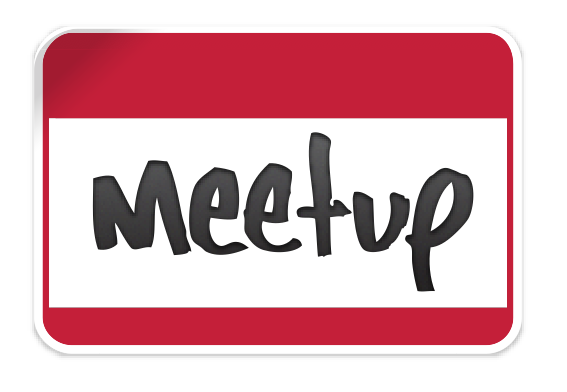
\includegraphics{logo.png}}
\note{if you're here, you probably know Meetup at least vaguely.}

\takahashi{12,604}
\note{Meetups today (Sunday is better)}

\takahashi{140,916}
\note{total Meetup Groups}

\takahashi{262,080}
\note{members on Android, 30d}

\takahashi{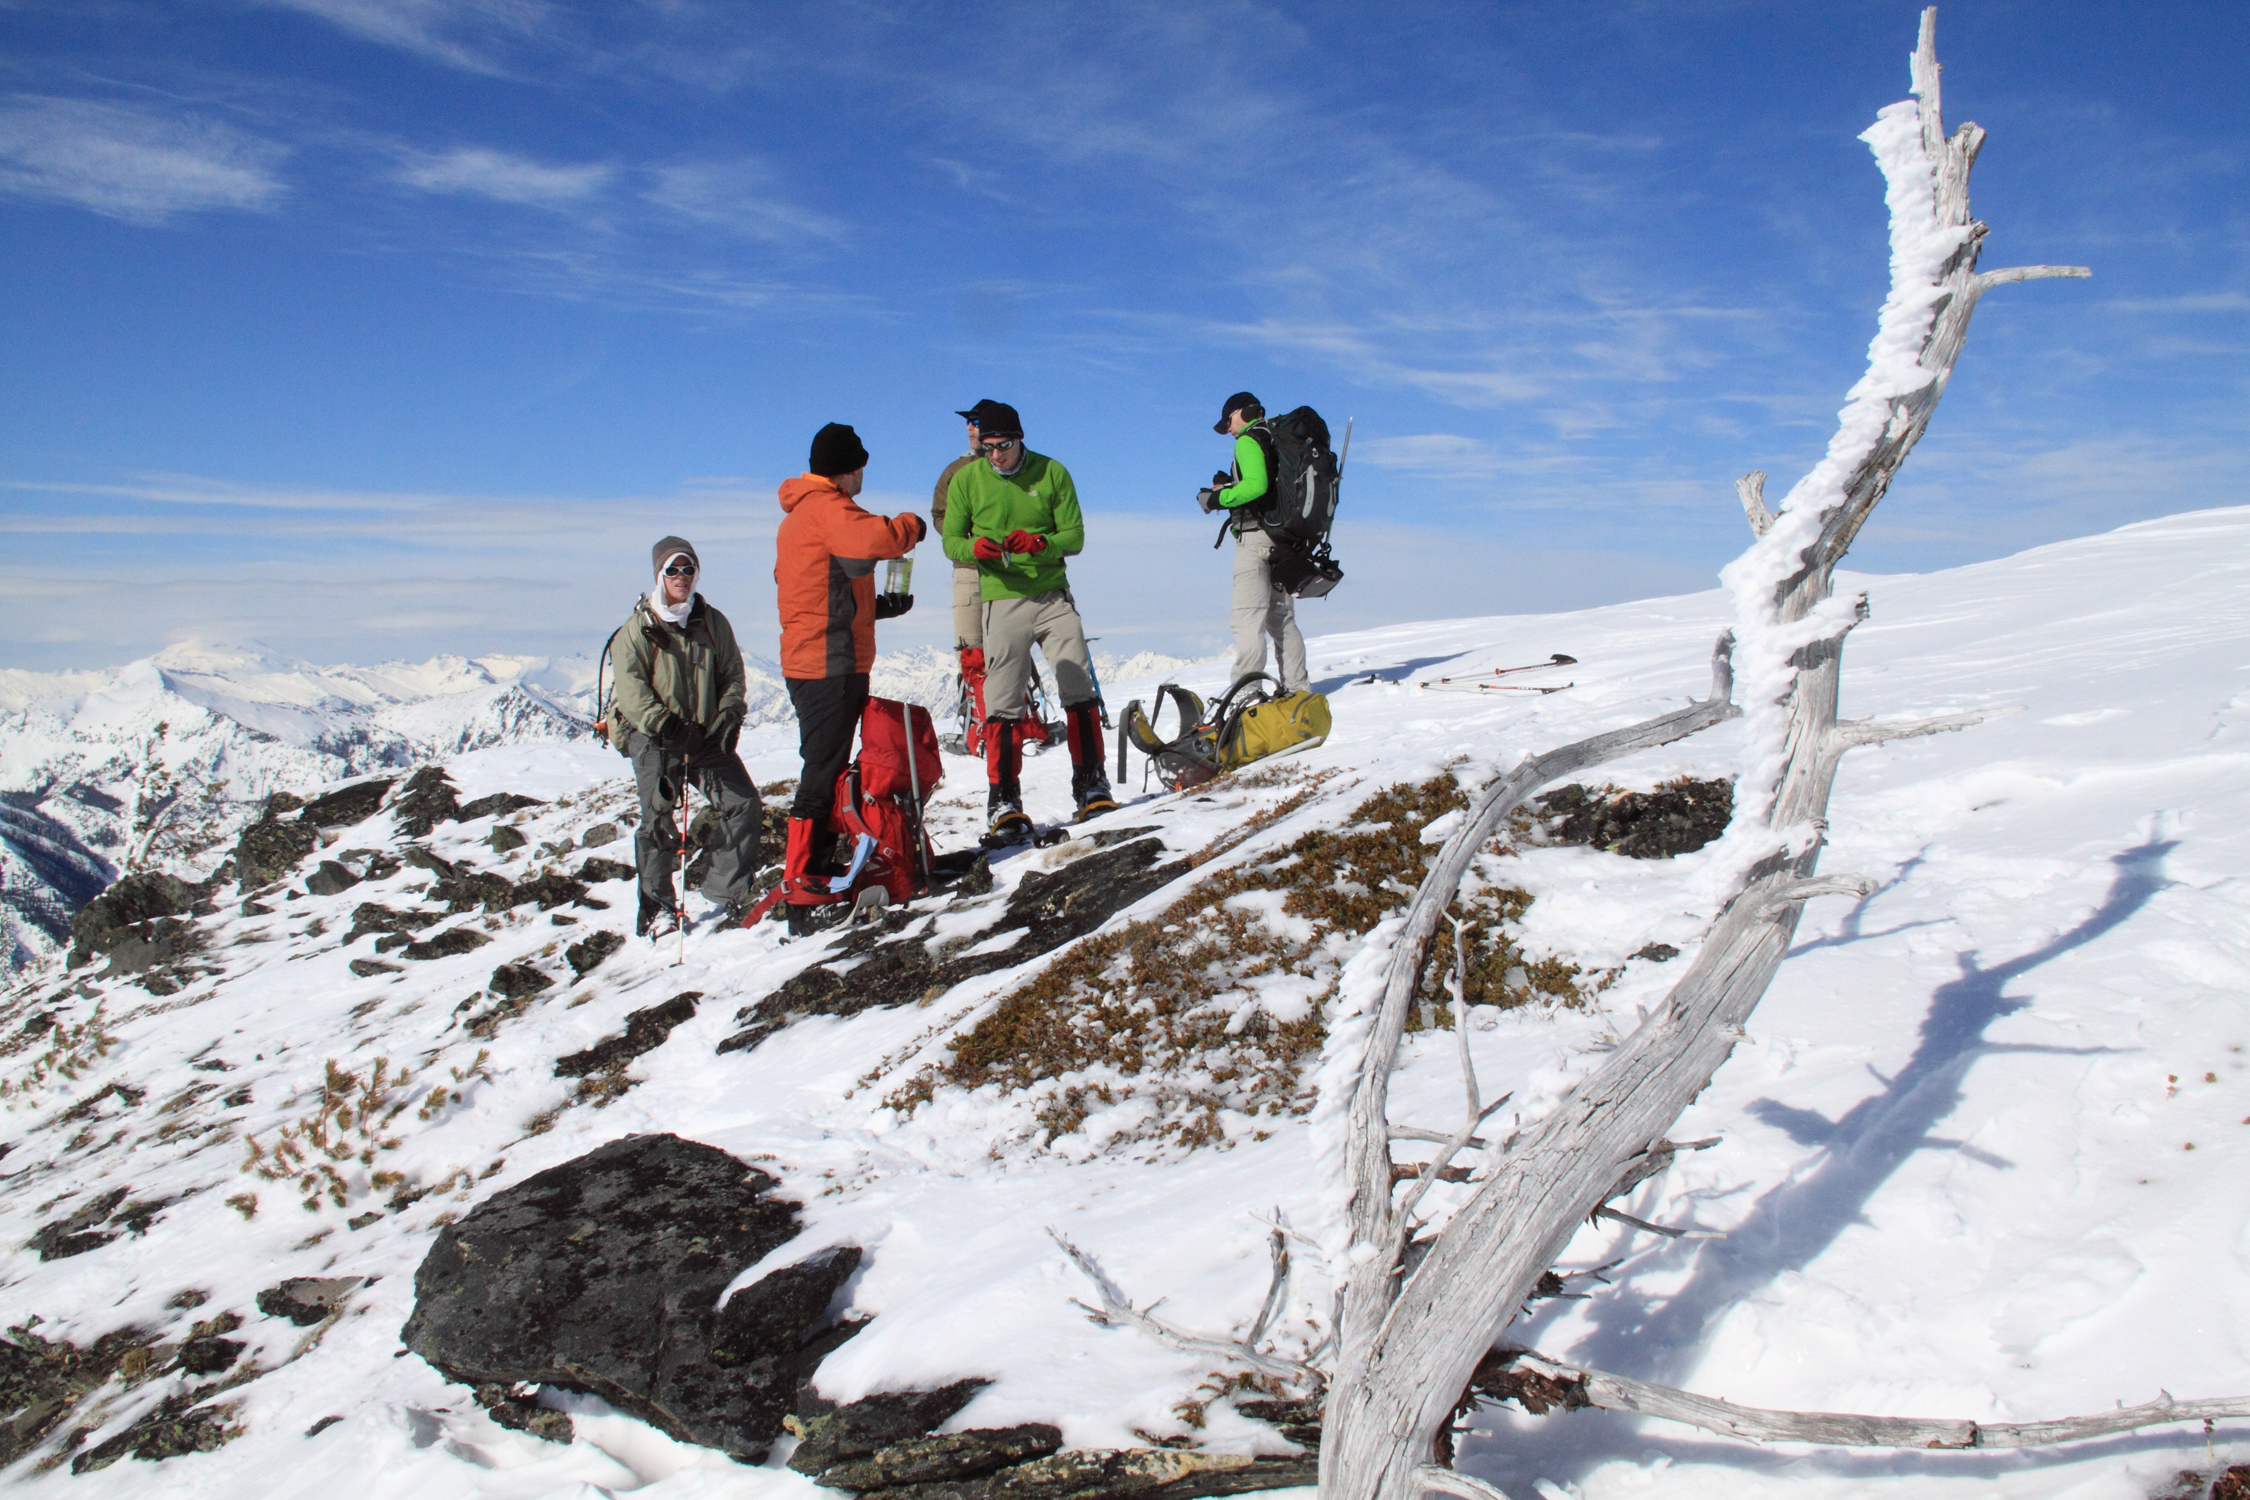
\includegraphics{highres_104595152.jpeg}}
\note{HERE ARE SOME CHALLENGES with our data. Peaks Adventures, Seattle. This is the kind of photo we always
throw in presentations, and isn't it beautiful? But: I don't live in
Seattle, and I don't ski.}

\takahashi{http://meetup.github.io/stream/rsvpTicker/}
\note{RSVP ticker demo}

\takahashi{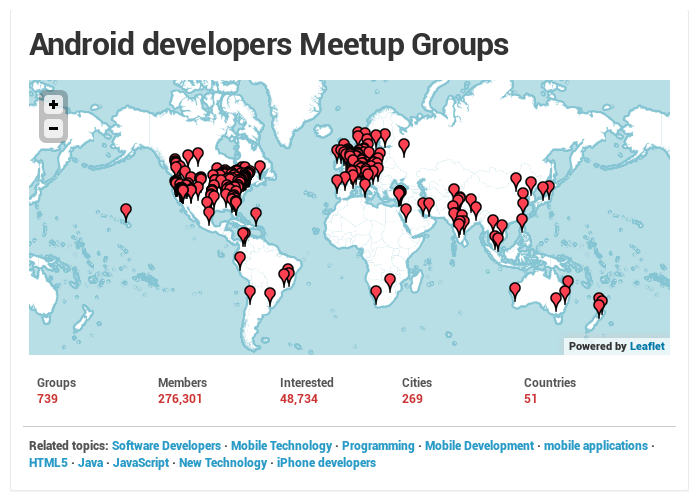
\includegraphics{android-meetups.png}}
\note{locality matters}

\takahashi{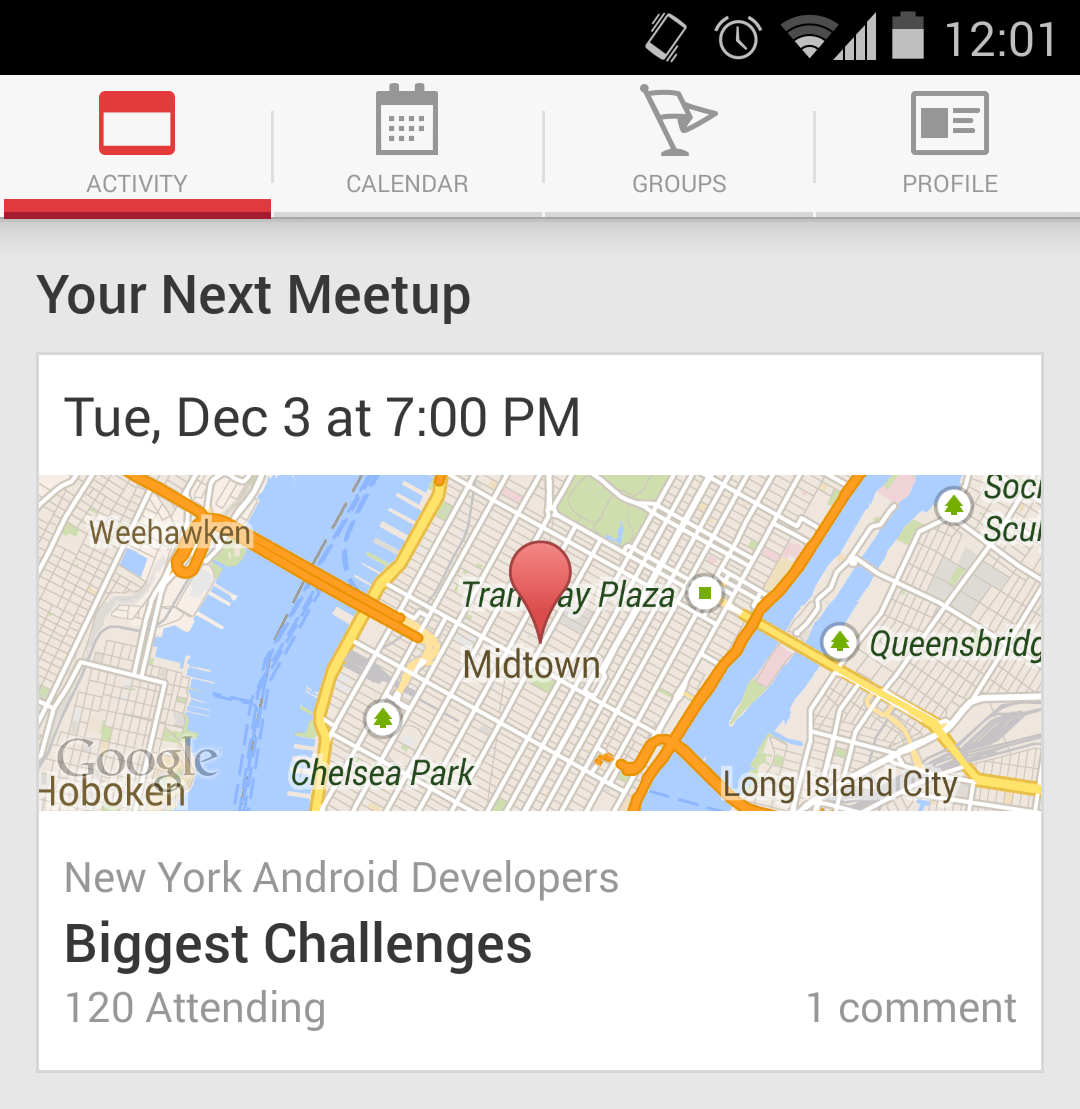
\includegraphics{mup-for-android.png}}
\note{personalization matters}

\takahashi{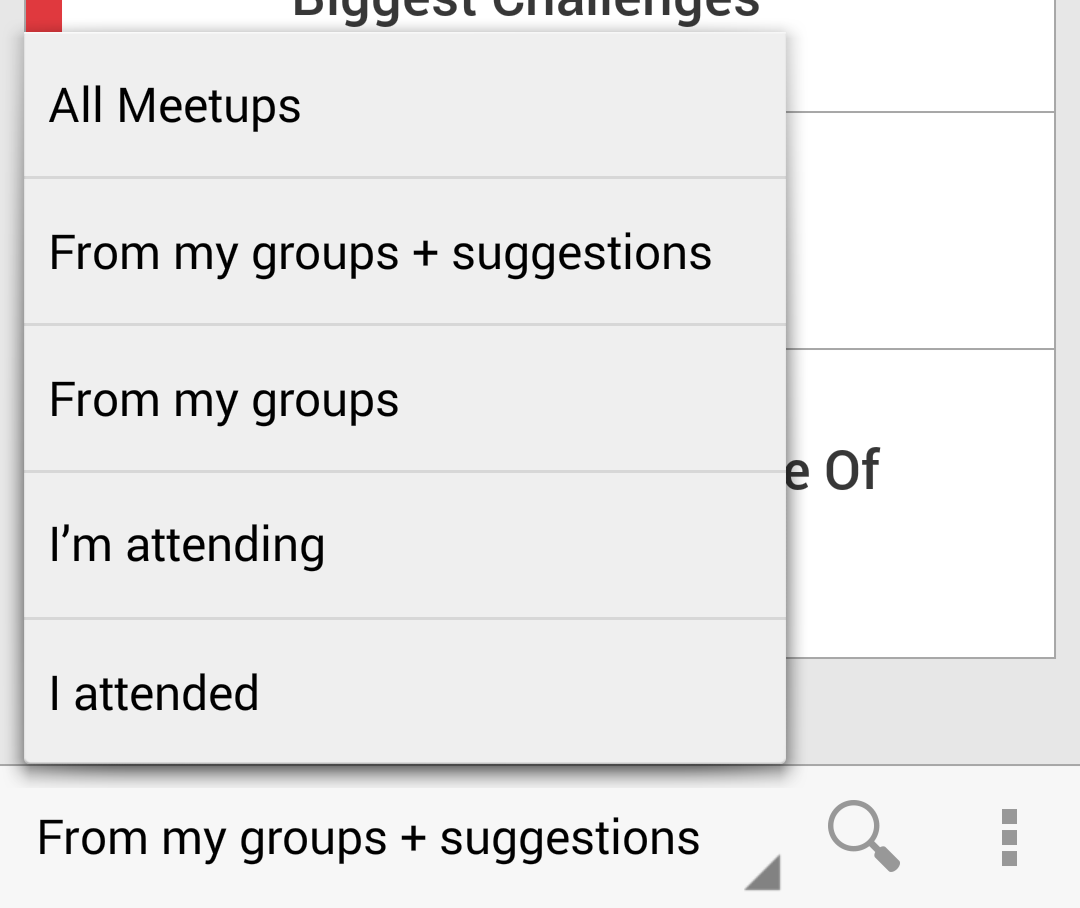
\includegraphics{calendar-view.png}}
\note{data is subset of other data: single event is $\subseteq$ of event
  list; MUPs I'm attending $\subseteq$ upcoming in my groups,…}

\takahashi<1-3>[label=wld]{\stack{Dataflow\onslide<2-5>{:}\\\onslide<2,4>{Win}\onslide<2>{, }\onslide<2,5>{Lose}\onslide<2>{,\\or }\onslide<2,3>{Draw}%
\note<1>{how do we get the right data to our Members' devices,
  maximizing accuracy while minimizing latency?}}}

\takahashi{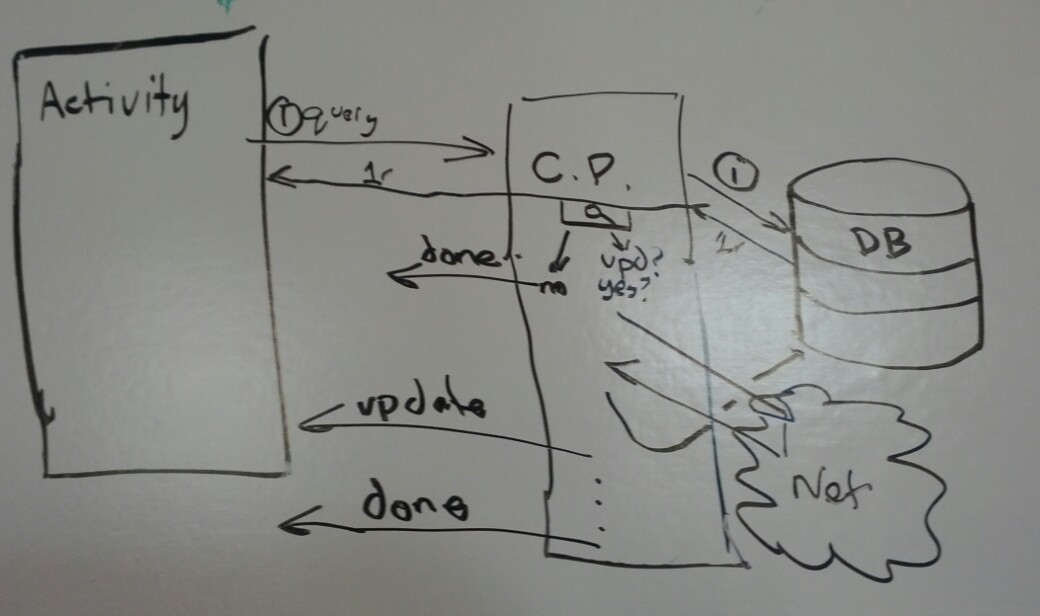
\includegraphics{diagram.jpeg}}
\note{\begin{itemize}
\item maybe could have drawn this better
\item \texttt{Activity} (or \texttt{Fragment}) asks Content Provider
  for data; uses Loader
\item CP returns ``immediately'' with data in local SQLite cache
\item CP decides if a network call is needed, tells network Service if
  so
\item network service calls back into CP with new data,
\item contentobservable magic causes Loader to requery…
\item new data!
\end{itemize}}

\againframe<2,4>{wld}

\takahashi{\stack{\texttt{\$ git diff --stat 1.2.2..dataflow\_30116 | tail -1}\\
\texttt{239 files changed, 6124 insertions(+), 10936 deletions(-)}}}
\note{less code}

\takahashi{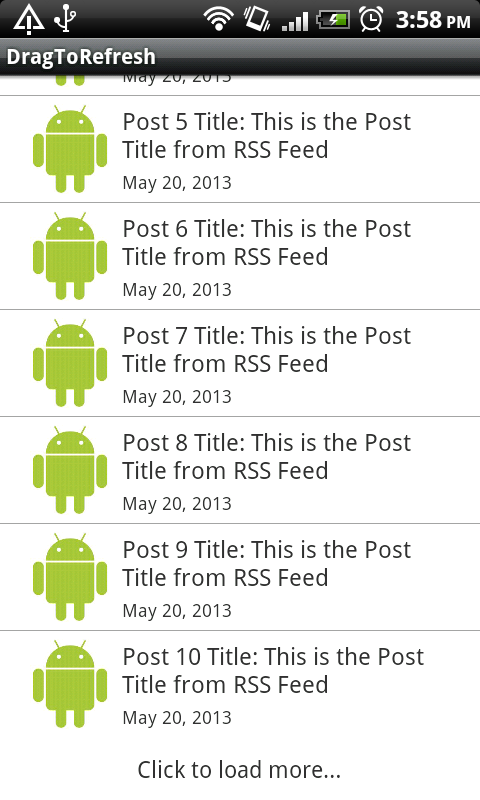
\includegraphics{load-more.png}}
\note{I dunno, some random graphic from the Internet, but anyway we don't have this}

\begin{frame}[fragile]
\begin{lstlisting}
/* almost ORM-like queries */
Query.getPhotosByEventId(eventId).loader(activity, PHOTO_COLS, "created DESC");
Query.getMemberEventsByTime(EPOCH, now).loader(this, PROJECTION, Query.REVERSE_TIME_ORDER);
\end{lstlisting}
\end{frame}

\againframe<2,5>{wld}

\begin{frame}[fragile]
\note{in content provider}
\begin{lstlisting}
private Intent getLoadIntent(String table, String selection, String[] select
ionArgs, String sortOrder) {
  if ("events".equals(table)) {
    if (byRid) {
      intent = API.Event.eventDetails(rid);
    } else if (Query.MEMBER_PAST_TIME.equals(selection) || Query.MEMBER_FUTURE_TIME.equals(selection)) {
      // ...
\end{lstlisting}
\end{frame}

\begin{frame}[fragile]
\note{in http service}
\begin{lstlisting}
public static Parser createParser(Context context, Intent intent) {
  final Uri uri = intent.getData();
  UriMatcher matcher = MATCHERS.get(method);
  switch (matcher.match(uri)) {
    case GET_EVENTS:
      String eventId = extractStringParam(intent, "event_id");
      // ...
\end{lstlisting}
\end{frame}

\takahashi{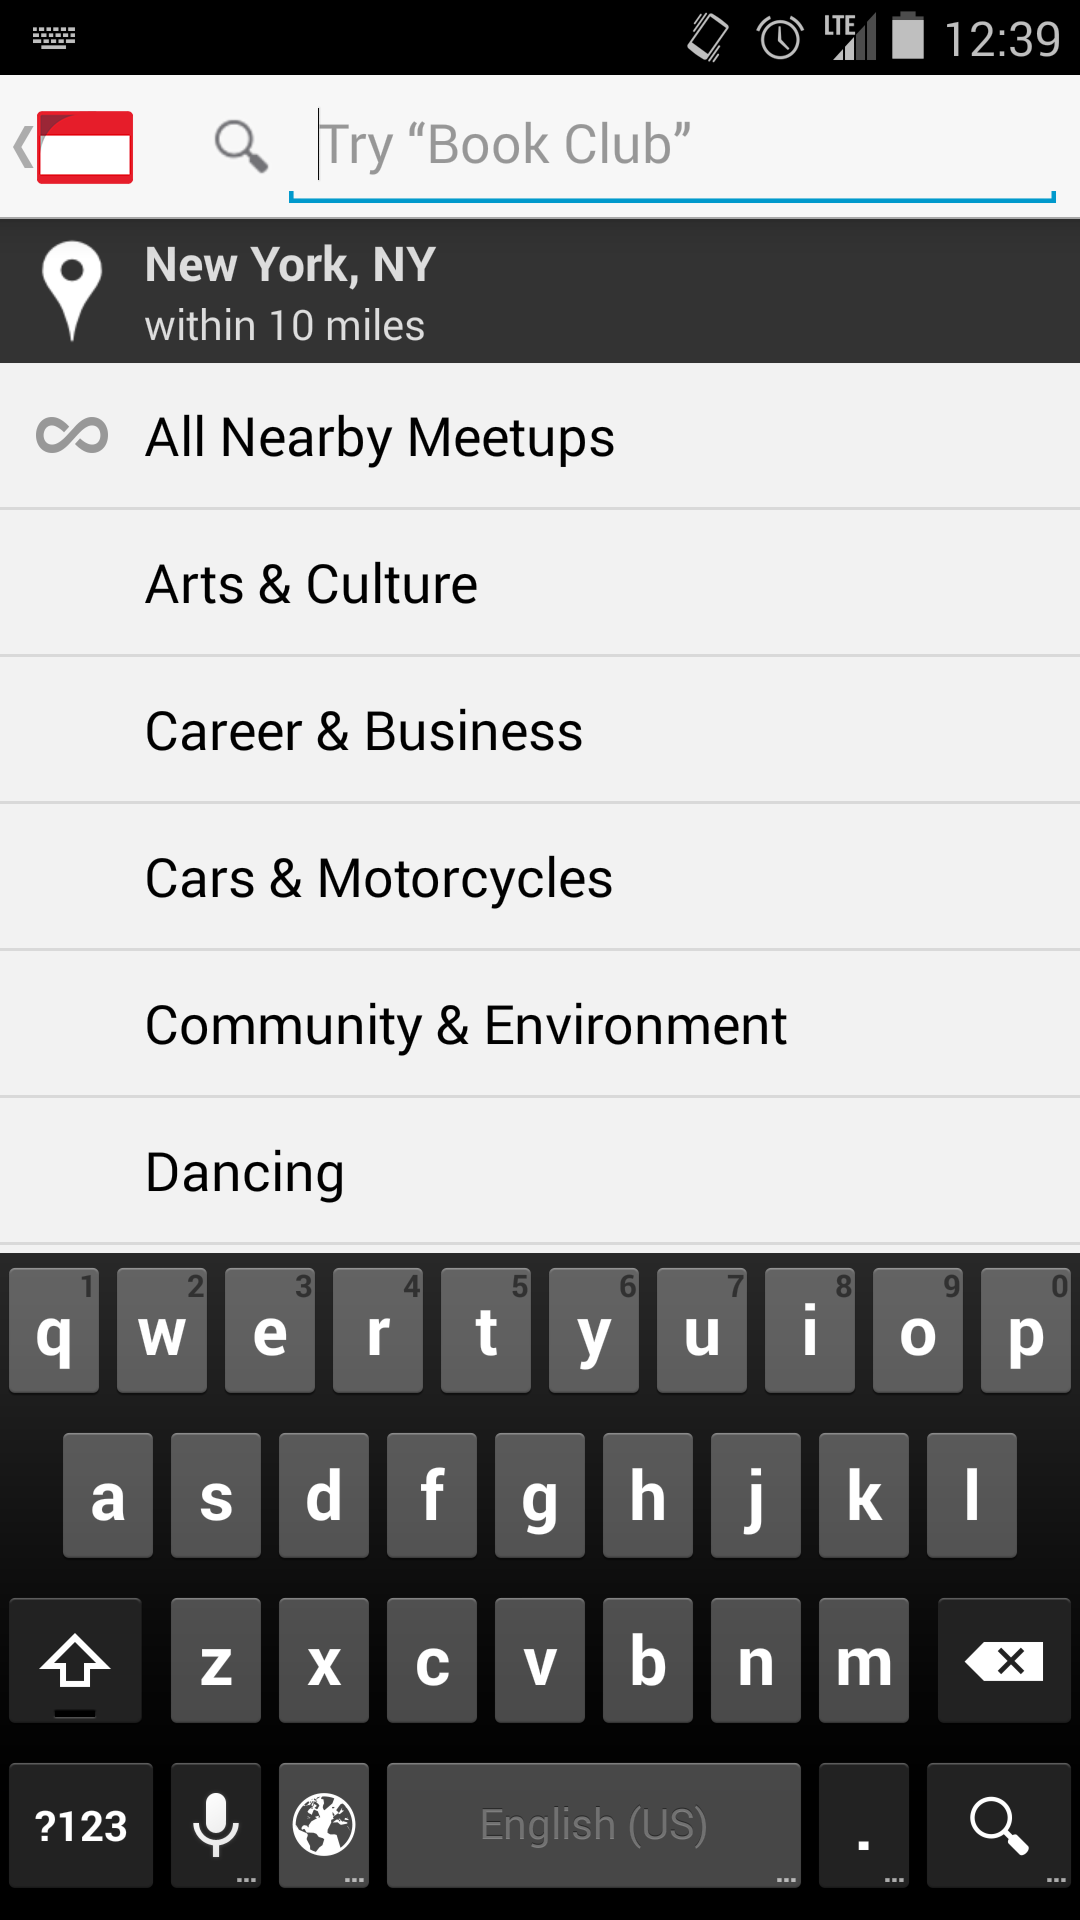
\includegraphics{search.png}}
\note{arbitrary queries can mess with things}

\takahashi{
\includegraphics{rsvp.png}}
\note{\begin{itemize}
\item POST vs GET
\item UI calls HTTP service directly
\item ResultReceiver, etc.
\item (still: data ends up in DB)
\end{itemize}}

\begin{frame}
\note{like everybody else, we're hiring}
\frametitle{Stay in touch}
\begin{itemize}
\item Email: \texttt{mlc@meetup.com}
\item Twitter: \texttt{@vermicelli}
\end{itemize}
\end{frame}
\end{document}
